%! TeX program = lualatex
\documentclass[a4paper, 10pt]{article} 
\usepackage[a4paper, margin=1.5cm]{geometry}

% packages
\usepackage{microtype}      % Slightly tweak font spacing for aesthetics
\usepackage[english]{babel} % Language hyphenation and typographical rules
\usepackage[final, colorlinks = true, urlcolor = black, linkcolor = black, citecolor = black]{hyperref} 
\newcommand{\secref}[1]{\textbf{§\ref{#1}~\nameref{#1}}}
\usepackage{changepage}     % adjust margins on the fly
\usepackage{multicol}

\usepackage[backend=biber, style=numeric, date=iso, urldate=iso]{biblatex}
\addbibresource{references.bib}
\DeclareFieldFormat{urldate}{Accessed on: #1}

\usepackage{fontspec}
\setmainfont{EB Garamond}
\setmonofont[Scale=MatchLowercase]{Deja Vu Sans Mono}

\usepackage{minted}
\usemintedstyle{algol_nu}
\usepackage{xcolor}

\usepackage{pgfplots}
\pgfplotsset{width=\textwidth,compat=1.9}

\usepackage{caption}
\newenvironment{code}{\captionsetup{type=listing}}{}
\captionsetup[listing]{skip=0pt}
\setlength{\abovecaptionskip}{5pt}
\setlength{\belowcaptionskip}{5pt}

\usepackage[yyyymmdd]{datetime}
\renewcommand{\dateseparator}{--}

\usepackage{tikz}
\usetikzlibrary{trees}

\usepackage{titlesec}
% \titleformat{\section}{\LARGE\bfseries}{}{}{}[\titlerule]
% \titleformat{\subsection}{\Large\bfseries}{}{0em}{}
% \titlespacing{\subsection}{0em}{-0.7em}{0em}
%
% \titleformat{\subsubsection}{\large\bfseries}{}{0em}{$\bullet$ }
% \titlespacing{\subsubsection}{1em}{-0.7em}{0em}

% margins
% \addtolength{\hoffset}{-2.25cm}
% \addtolength{\textwidth}{4.5cm}
% \addtolength{\voffset}{-3.25cm}
% \addtolength{\textheight}{5cm}
\setlength{\parskip}{0pt}
\setlength{\parindent}{0in}
% \setcounter{secnumdepth}{0}

\begin{document}
\hrule \medskip
\begin{minipage}{0.295\textwidth} 
    \vfill
    \raggedright
    \footnotesize 
    \begin{tabular}{@{}l l} % Define a two-column table with left alignment
        Name: & Andrew Hayes \\
        Student ID: & 21321503 \\
        Programme: & 4BCT \\
    \end{tabular}
    \vfill
\end{minipage}
\begin{minipage}{0.4\textwidth} 
    \centering 
    \Large 
    \vfill
    \textbf{CT4101}
    \vfill
\end{minipage}
\begin{minipage}{0.295\textwidth} 
    \raggedleft
    \vfill
    \today
    \vfill
\end{minipage}
\smallskip
\hrule 
\begin{center}
    \normalsize
    Assignment 1: Classification Using Scikit-Learn
\end{center}
\hrule

% \begin{multicols}{2}
% \fontsize{9}{9}\selectfont
% \begin{multicols}{2}
\section{Description of Algorithms}
\subsection{Algorithm 1: Random Forest}
% Detailed description of algorithm 1.
% Clearly describe each of your chosen scikit-learn algorithm implementations in turn, paying special attention to discussing the two hyperparameters that you have chosen to tune for each algorithm.
% You should write a maximum of 1 page per algorithm. 

\textbf{Random decision forest} is a supervised machine learning algorithm that can be used for both classification \& regression that builds upon the \textbf{decision tree} algorithm by combining several decision trees to generate labels for a dataset.
An implementation of this algorithm for classification is provided in scikit-learn as \mintinline{python}{sklearn.ensemble.RandomForestClassifier} \supercite{scikit_randomforestclassifier}.
While it can be used for regression as well as classification, I will only be referring to its use as a classification algorithm in this assignment, as regression is not relevant to the wildfire classification task at hand.
\\\\
Since the random decision forest algorithm builds upon the decision tree algorithm, it is first necessary to explain briefly what decision trees are and how they work.
A decision tree can be thought of a series of internal nodes (i.e., nodes which are not leaf nodes) that contain a question which separates the input data.
The decision tree is traversed from root to leaf for each instance being classified, where the leaf node to which we arrive is the label for that instance.
For example, a decision tree might be used to determine whether or not a living thing is a mammal, where each internal node is a question that helps to separate non-mammalian data instances from mammalian, and each leaf node is a label stating whether or not the living thing is a mammal.
Each internal node should narrow down the final label as much as possible i.e., each question should give us the maximum information about the instance and should be arranged in the order that narrows it down as quickly as possible.

\begin{figure}[H]
    \centering
    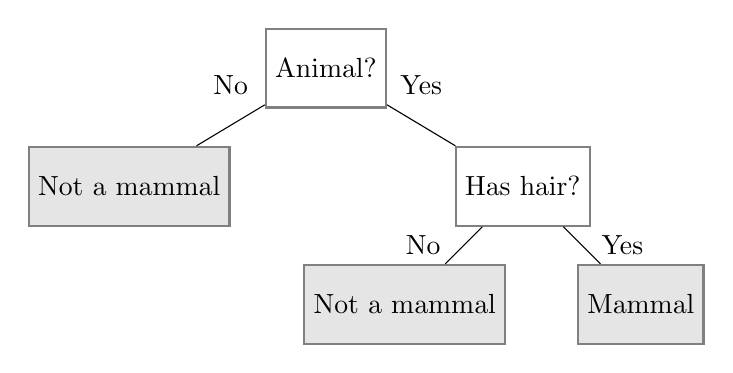
\begin{tikzpicture}[
        every node/.style={rectangle, draw=black!50, thick, minimum size=1cm},
        level 1/.style={sibling distance=5cm},
        level 2/.style={sibling distance=3cm}
    ]

    % Internal Nodes
    \node[fill=white] {Animal?}
        child { node[fill=gray!20] {Not a mammal}  edge from parent node[above, draw=none] {No} }
        child { node[fill=white] {Has hair?}
            child { node[fill=gray!20] {Not a mammal} edge from parent node[left, draw=none] {No} }
            child { node[fill=gray!20] {Mammal} edge from parent node[right, draw=none] {Yes} }
            edge from parent node[above, draw=none] {Yes}
        };

    \end{tikzpicture}
    \caption{Simplified Decision Tree to Determine Whether a Creature is a Mammal}
\end{figure}

Decision trees have many advantages: they are visualisable by humans and aren't ``black-box'', they can model non-linear relationships easily, and they are robust to outliers.
However, they have their disadvantages, including instability (small changes in the training data can significantly alter the tree structure) and in particular \textbf{overfitting}: when the algorithm fits too exactly to the training data, making it incapable of generalising to unseen data.
An extreme example of overfitting would be if the example decision tree above started to ask far too specific questions, e.g. ``Is it a dolphin'', ``Is it a human''. 
While this would have excellent performance \& accuracy on the test data, it would not work at all for an animal it hadn't encountered before.
\\\\
Random forests work by combining many decision trees into a forest, thus improving accuracy \& reducing overfitting by averaging multiple trees, reducing variance and leading to better generation.
These decision trees are each generated using random, potentially overlapping subsets of the data training data.
While the original random forest algorithm worked by taking the most popular label decided on by the set of trees \supercite{breiman}, the scikit-learn \mintinline{python}{RandomForestClassifier} works by taking a probability estimate for each label from each tree and averaging these to find the best label\supercite{scikit_ensembles}.
\\\\
In \mintinline{python}{RandomForestClassifier}, each tree is generated as follows:
\begin{enumerate}
    \item   A subset of the training data is randomly selected (hence the ``Random'' in the name of the algorithm).
            These subsets are selected ``with replacement'' which means that different trees can select the same samples: they are not removed from the pool once they are first selected.
            This results in unique, overlapping trees.
    \item   Starting with the root node, each node is \textit{split} to partition the data.
            Instead of considering all features of the samples when choosing the split, a random subset of features is selected, promoting diversity across the trees.
            The optimal split is calculated using some metric such as Gini impurity or entropy to determine which split will provide the largest reduction in impurity.
    \item   This process is repeated at every node until no further splits can be made.
\end{enumerate}

\begin{figure}[H]
\centering
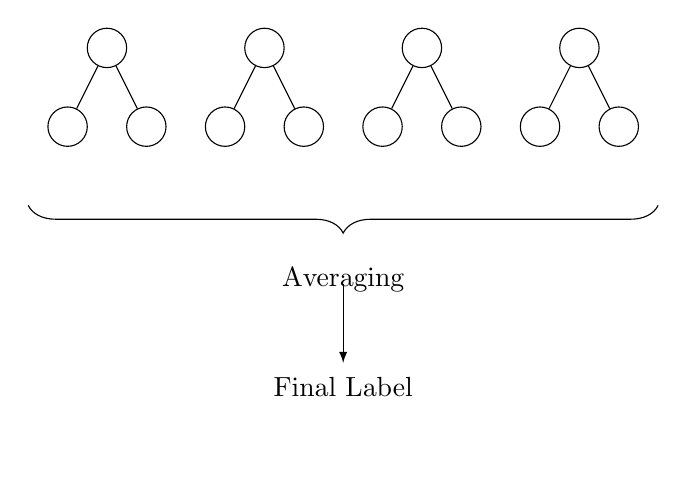
\begin{tikzpicture}[every node/.style={circle, draw, minimum size=0.5cm}]

    % Binary Trees
    \node (tree1) at (0,0) {};
    \node (tree1l) at (-0.5,-1) {};
    \node (tree1r) at (0.5,-1) {};
    \draw (tree1) -- (tree1l) {};
    \draw (tree1) -- (tree1r) {};
    
    \node (tree2) at (2,0) {};
    \node (tree2l) at (1.5,-1) {};
    \node (tree2r) at (2.5,-1) {};
    \draw (tree2) -- (tree2l) {};
    \draw (tree2) -- (tree2r) {};

    \node (tree3) at (4,0) {};
    \node (tree3l) at (3.5,-1) {};
    \node (tree3r) at (4.5,-1) {};
    \draw (tree3) -- (tree3l) {};
    \draw (tree3) -- (tree3r) {};
    
    \node (tree4) at (6,0) {};
    \node (tree4l) at (5.5,-1) {};
    \node (tree4r) at (6.5,-1) {};
    \draw (tree4) -- (tree4l) {};
    \draw (tree4) -- (tree4r) {};

    % Averaging Bracket
    \draw[decorate,decoration={brace,amplitude=10pt,mirror}] (-1,-2) -- (7,-2) node[below, midway, draw=none] {Averaging};

    % Final Label
    % \node at (4,-3) {final label};
    % \draw[->] (4,-2) -- (4,-2.5);
    \draw[-latex] (3,-3) -- (3,-4); % Adjust the coordinates as needed
    \node[draw=none] at (3,-4.3) {Final Label};
\end{tikzpicture}
\caption{Random Forest Algorithm Example Diagram (with scikit-learn Averaging)}
\end{figure}

I chose the random forest classifier because it is resistant to overfitting, works well with complex \& non-linear data like the wildfire data in question, handles both categorical \& numerical features, and offers a wide variety of hyperparameters for tuning.
It also has many benefits that are not particularly relevant to this assignment but are interesting nonetheless: it can handle both classification \& regression tasks, can handle missing data, and can be parallelised for use with large datasets.

\subsubsection{Hyperparameter 1: \mintinline{python}{n_estimators}}
The hyperparameter \mintinline{python}{n_estimators} is an \mintinline{python}{int} with a default value of 100 which controls the number of decision trees (\textit{estimators}) in the forest\supercite{scikit_randomforestclassifier}.
Increasing the number of trees in the forest generally improves the model's accuracy \& stability, with diminishing marginal returns past a certain value, at the trade-off of increased computation \& memory consumption.
Each tree is independently trained, so there is a big trade-off between computational cost \& performance.
Using a lower number of estimators can result in underfitting, as there may not be a enough trees in the forest to capture the complexity of the data.

\subsubsection{Hyperparameter 2: \mintinline{python}{max_depth}}
The hyperparameter \mintinline{python}{max_depth} is an \mintinline{python}{int} with a default value of \mintinline{python}{None} which controls the maximum ``depth'' of each of the trees in the forest \supercite{scikit_randomforestclassifier}, where the ``depth'' of a tree refers to the longest path from the root node to a leaf node in said tree.
With the default value of \mintinline{python}{None}, the trees will continue to grow until they cannot be split any further, meaning that each leaf node either only contains samples of the same class (i.e., in our case each leaf node is a definitive ``yes'' or ``no'') or contains a number of samples lower than the \mintinline{python}{min_samples_split} hyperparameter.
The \mintinline{python}{min_samples_split} hyperparameter determines the minimum amount of samples needed for a node to be split; it has a default \mintinline{python}{int} value of 2 and therefore, since I am not tuning this hyperparameter for this assignment, it has no relevance as any leaf node that doesn't reach the minimum amount of samples to be split is a ``pure'' node by virtue of containing only one class.
\\\\
High \mintinline{python}{max_depth} values allow for the trees to capture more complex patterns in the data, but can overfit the data, leading to poor testing accuracy.
Bigger trees also naturally incur higher computational costs, requiring both more computation to create and more memory to store. 
Lower \mintinline{python}{max_depth} values result in simpler trees which can only focus on the most important features \& patterns in the data, which in turn can reduce overfitting;
however, low values run the risk of creating trees which are not big enough to capture the complexity of the data, and can lead to underfitting.

\subsection{Algorithm 2: C-Support Vector Classification}
\textbf{C-Support Vector Classification} is a supervised machine learning algorithm provided in scikit-learn as \mintinline{python}{sklearn.svm.SVC}, as it is a \textbf{Support Vector Machine (SVM)} based algorithm.
It is capable of performing both binary \& mutli-class classification, on both linearly and non-linearly separable data. 
While SVMs can also be used for regression as well as classification, I will only be considering their use in classification for this assignment.
\\\\
SVM is a supervised learning algorithm that works by constructing a hyperplane in a multidimensional space that separates each data sample into a distinct class, i.e. it draws a ``line'' in $N$ dimensions (where $N$ is the number of features) that separates all the samples in one class from all the samples in the others.
In mathematical terms, the data samples in this high-dimensional space are \textit{vectors}, as the value of each feature for that sample determines the direction \& magnitude of the object representing the sample in that space.
The vectors closest to the boundary hyperplane are called \textbf{support vectors}: they are called this because they \textit{support} the boundary between the two classes, as the algorithm is always trying to maximise the distance on either side of the boundary between the boundary and the nearest data samples.
The further the decision boundary is from the outermost data points in each class, the more generalisable the classifier will be.
This also reduces overfitting, as a decision boundary that is closely defined by specific data points will be highly sensitive to noise in the data \& outliers, as a data point that is just a little bit away from another data point in its class could happen to be on the wrong side of the boundary and get misclassified.
\\\\
However, if the data is not linearly separable, something called the \textbf{kernel trick} is employed.
This is where data that is not linearly separable in its original $N$-dimensional space is mapped to a higher dimensional space where a hyperplane that delineates the two classes can be found.
To find the similarity of two support vectors $x$ \& $y$ without the kernel trick, we would have to calculate the dot product $\phi(x) \cdot \phi(y)$ where $\phi$ is some function that maps the data to a higher dimensional space, which is computationally expensive.
The kernel trick avoids this by using some kernel function $K$ which calculates the dot product in the higher dimensional space without having to first map the data to that higher dimensional space, so $K(x,y) = \phi(x) \cdot \phi(y)$.

\subsubsection{Hyperparameter 1: \mintinline{python}{kernel}}
The hyperparameter \mintinline{python}{kernel} specifies the kernel function to be used when employing the kernel trick.
The possible values are:\supercite{scikit_kernel}
\begin{itemize}
    \item   \mintinline{python}{"linear"}: Assumes that the data is linearly separable, and does not transform it into a higher dimension, instead just directly computing the dot product $K(x,y) = x \cdot y$.

    \item   \mintinline{python}{"poly"}: Calculates the polynomial of the features of data sample and considers the polynomial relationships as well as the linear relationships between the data samples.
            The formula for this kernel is $K(x,y) = (x \cdot y + c)^d$ where $c$ is a constant \& $d$ is the degree of the polynomial.

    \item   \mintinline{python}{"rbf"}: The Radial Basis Function (also called the Gaussian kernel) calculates the similarity between the data samples in infinite dimensions.
            The formula for this kernel is $K(x, y) = \exp(- \gamma \cdot || x - y ||^2)$ where $\gamma$ determines the \textit{width} of the kernel (how far the influence of a data sample reaches).
            This is the default kernel for the \mintinline{python}{sklearn.svm.SVC} class.

    \item   \mintinline{python}{"sigmoid"}: Calculates the similarity between the data samples using the hyperbolic tangent function, which creates an S-shaped curve called a \textit{sigmoid} and determines which side of the sigmoid a data target is on to classify it.
            The formula for this function is $K(x,y) = \tanh (\gamma \cdot x \cdot y + r)$ where $\gamma$ controls the influence of a data sample as before and $r$ controls a bias that shifts the boundary defined by the sigmoid function to be more or less lenient.

    \item   \mintinline{python}{"precomputed"}: Instead of specifying a kernel function to use on the data, one can specify a matrix that contains the pre-computed kernel function output of your choosing, which can save calculations being performed twice.
\end{itemize}


\subsubsection{Hyperparameter 2: \mintinline{python}{C}}
The hyperparameter \mintinline{python}{C} is called the \textbf{regularisation parameter} because it controls how misclassified samples are penalised, i.e. controlling how ``regularised'' or smooth the boundary hyperplane is.
It is a \mintinline{python}{float} with a default value of 1.0.
A higher value for \mintinline{python}{C} will result in misclassifications being heavily penalised, which in the extreme case will results in the model prioritising correctly classifying each data sample over having a wider margin, which can make the model less generalisable and cause overfitting.
On the other hand, a lower value for \mintinline{python}{C} will result in a model that has a greater acceptance of misclassifications in return for a wider margin, which can improve generalisability but reduce precision.

\section{Model Training \& Evaluation}
I chose to write the Python code to train \& evaluate the models in a Jupyter notebook in Google Colab: I used a Jupyter Notebook just for the easy rendering of plots within the IDE and I used Google Colab to have access to faster hardware than my own.
For the hyperparameter tuning of both algorithms, I created an array of values for each hyperparameter that were iterated over in a nested \mintinline{python}{for} loop, and created a heatmap of the accuracy results.

\subsection{Algorithm 1: Random Forest}\label{sec:foresteval}
Since the Random Forest algorithm can handle categorical features, the dataset had no missing data, and random forests don't require feature scaling, I did not perform any pre-processing for this algorithm.
The first thing I did was train a \mintinline{python}{RandomForestClassifier} with the default parameters as a control variable to which I could compare my hyperparameter tuning.
The only thing I changed from default for this was that I set the random seed \mintinline{python}{random_state = 0} so that I would get the same reproducible output for the same code, regardless of how many times it was ran as otherwise it would be exceedingly difficult to draw meaningful comparison between the subsequent runs of the algorithm.
While this is a parameter that is supplied to the model, it is not a \textit{hyperparameter} as it does not control the behaviour of the model in terms of learning or performance; it cannot be tuned, and there is no optimal value. 
% \end{multicols}

\begin{minipage}{0.45\textwidth} 
\begin{figure}[H]
    \centering
    \includegraphics[width=\textwidth]{./images/randomforestclassifier_defaulthyperparameters_confusionmatrix.png}
    \caption{Confusion Matrix}
\end{figure}
\end{minipage}\hspace{0.05\textwidth}
\begin{minipage}{0.45\textwidth} 
\begin{code}
\begin{minted}[frame=none]{text}

Training Accuracy: 1.0000
Classification Report of Testing Results:
              precision    recall  f1-score   support

          no       1.00      1.00      1.00        75
         yes       1.00      1.00      1.00        79

    accuracy                           1.00       154
   macro avg       1.00      1.00      1.00       154
weighted avg       1.00      1.00      1.00       154
\end{minted}
\caption{Training Accuracy \& Classification Report}
\end{code}
\begin{code}
\begin{minted}[frame=none]{text}
Testing Accuracy: 0.8200
Classification Report of Testing Results:
              precision    recall  f1-score   support

          no       0.76      0.86      0.81        22
         yes       0.88      0.79      0.83        28

    accuracy                           0.82        50
   macro avg       0.82      0.82      0.82        50
weighted avg       0.83      0.82      0.82        50
\end{minted}
\caption{Testing Accuracy \& Classification Report}
\end{code}
\end{minipage}

When I was tuning the hyperparameter values, I noticed that the algorithm seemed to be performing very well with low values of \mintinline{python}{n_estimators} \& \mintinline{python}{max_depth} so the array of values tested starts with very small increments between the values, and then grows into quite large increments at the end.
\begin{figure}[H]
    \centering
    \includegraphics[width=0.7\textwidth]{./images/randomforestclassifier_hyperparamtuning.png}
    \caption{Accuracy Heatmap}
\end{figure}

I obtained a training accuracy of 100\% using the default hyperparameter values: this indicates overfitting, and we saw that the accuracy did drop on the test data to 82\%.
The most likely cause of this overfitting is that \mintinline{python}{max_depth} defaults to \mintinline{python}{None}, which can create very complex trees that perform well on the training data, but aren't generalisable to unseen data.
\\\\
The hyperparameter tuning results were very surprising to me.
The accuracy results obtained were not that unusual: we obtained a +4\% increase for our maximum accuracy value, going from 82\% to 86\%, and the lowest accuracy we obtained was 80\%, indicating that the model's performance was stable across a range of hyperparameters.
It was surprising that 10 proved to be the optimal value of \mintinline{python}{n_estimators} for this dataset, as this is significantly lower than the default value of 100, and a higher number of estimators typically results in improved accuracy \& stability.
My hypothesis is that the low number of trees in the forest helped to prevent overfitting caused by the relatively high \mintinline{python}{max_depth}.
We can see from the data that for a low \mintinline{python}{max_depth = 1}, higher \mintinline{python}{n_estimators} yield better accuracy, which supports my idea that the low number of trees is helping to prevent overfitting by the deep, complex trees.
It looks like that a relatively small \mintinline{python}{max_depth} of 5 through to \mintinline{python}{None} was suitable when paired with \mintinline{python}{n_estimators = 10}, perhaps because the dataset was sufficiently small \& non-complex that a shallower tree could still capture its complexity.

\subsection{Algorithm 2: C-Support Vector Classification}
Since SVMs don't support categorical data, I first encoded the \mintinline{python}{fire} column to have numerical values using \mintinline{python}{OneHotEncoder}.
I didn't standardise the data as a pre-processing step as it appeared to be beyond the scope of this assignment (and I'm pushing the page limit on this assignment as is without including extra bits), but it is often important to do so, as SVMs are very sensitive to scale in the sample data.
As in \secref{sec:foresteval}, I first began with the default values as a control to which I could compare my tuning.

\begin{minipage}{0.45\textwidth} 
\begin{figure}[H]
    \centering
    \includegraphics[width=\textwidth]{./images/svc_confusion.png}
    \caption{Confusion Matrix}
\end{figure}
\end{minipage}\hspace{0.05\textwidth}
\begin{minipage}{0.45\textwidth} 
\begin{code}
\begin{minted}[frame=none]{text}

Training Accuracy: 0.5130
Classification Report of Training Results:
              precision    recall  f1-score   support

         0.0       0.00      0.00      0.00        75
         1.0       0.51      1.00      0.68        79

    accuracy                           0.51       154
   macro avg       0.26      0.50      0.34       154
weighted avg       0.26      0.51      0.35       154
\end{minted}
\caption{Training Accuracy \& Classification Report}
\end{code}
\begin{code}
\begin{minted}[frame=none]{text}
Testing Accuracy: 0.5600
Classification Report of Testing Results:
              precision    recall  f1-score   support

         0.0       0.00      0.00      0.00        22
         1.0       0.56      1.00      0.72        28

    accuracy                           0.56        50
   macro avg       0.28      0.50      0.36        50
weighted avg       0.31      0.56      0.40        50
\end{minted}
\caption{Testing Accuracy \& Classification Report}
\end{code}
\end{minipage}


\begin{figure}[H]
    \centering
    \includegraphics[width=0.7\textwidth]{./images/svc_heatmap.png}
    \caption{Accuracy Heatmap}
\end{figure}

We can see from the heatmap that \mintinline{python}{kernel = "linear"} is far superior to any other kernel function.
This indicates that our data is linearly separable.
However, it's worth noting that we are only looking at tuning two hyperparameters here: some of these kernels have additional hyperparameters, and likely could've performed better if they were tuned appropriately.
Looking at the row corresponding to the linear kernel function in the heatmap, we can also see a nice demonstration of the effect of different \mintinline{python}{C} values: the accuracy of the model steadily increases as we increase the penalty for misclassifications, but after a certain point our accuracy starts to decrease.
This is likely because the very high \mintinline{python}{C} values (100 and above) were causing a very narrow margin when the boundary was being drawn, causing overfitting, as the boundary was not generalisable and performed poorly on the unseen data.
The relatively high optimal value for \mintinline{python}{C} indicates that the test data is quite similar to the training data, as a narrow margin can be maintained without sacrificing accuracy in the test.
We can see that placing a weak penalty for misclassification naturally reduces accuracy.
What's interesting about this data is that the very high \mintinline{python}{C} values seem to be able to force an accurate boundary even for kernel functions that are unsuitable for this type of data.
\\\\
The confusion matrix for the model with the default hyperparameters is quite interesting: it seems that this model only ever produced the label ``yes'' and never ``no'', resulting in an ``accuracy'' of 51\%: if you only ever guess ``yes'' and the options are an equally distributed set of ``yes'' and ``no'', you'll be right about half the time, even if there's no logic to your guess.
Based off the hyperparameter tuning, we can see that this is because the default hyperparameter values for this model are very different to the optimal ones for our data.
Firstly, we can see that from the heatmap that the RBF kernel function performed quite poorly on our data: it was the second worst kernel function in terms of accuracy.
However, this is only half the story, as we can see that with a suitably high \mintinline{python}{C} value, we can obtain a reasonably high accuracy even with RBF.
Clearly, the default value of \mintinline{python}{C = 1.0} is far too low for our data (the optimal for RBF was 10,000).
This is may be in part due to the fact that I did not scale the data before training \& testing, and the high \mintinline{python}{C} value is helping to compensate for this.

\section{Conclusion}
\subsubsection{Key Findings}
The key findings for each algorithm are as follows:
\begin{itemize}
    \item   Random Forest:
            \begin{itemize}
                \item   Accuracy with default hyperparameter values: 82\%.
                \item   Accuracy with hyperparameter tuning: 86\%.
                \item   The model demonstrated overfitting with a training accuracy of 100\%, dropping to 82\% on the test data, indicating that the default values overfit the data.
                \item   Hyperparameter tuning revealed that a lower number of decision trees (\mintinline{python}{n_estimators = 10}) and a relatively small maximum depth (\mintinline{python}{max_depth = 5}) achieved the best balance between performance and computational efficiency, with an optimal test accuracy of 86\%.
                \item   The model's performance remained stable across different hyperparameters, showing that it is robust to small changes.
            \end{itemize}

    \item   C-Support Vector Classification:
            \begin{itemize}
                \item   Accuracy with default hyperparameter values: 56\%.
                \item   Accuracy with hyperparameter tuning: 92\%.
                \item   The model initially performed poorly with the default hyperparameters, yielding a testing accuracy of 56\%.
                \item   Tuning the C parameter (\mintinline{python}{C = 100}) and using the linear kernel significantly improved performance, suggesting that the data is linearly separable.
                \item   The linear kernel consistently outperformed other kernel options, demonstrating its suitability for the dataset.
            \end{itemize}
\end{itemize}

Random Forest performed the best without any hyperparameter tuning, and its accuracy only slightly increased with tuning.
C-Support Vector Classification performed the best with hyperparameter tuning, achieving a quite respectable 92\% accuracy, despite having absolutely terrible performance with the default hyperparameter values.

\subsubsection{Recommended Hyperparameter Values Based Off Results}
Recommended hyperparameter values for Random Forest:
\begin{itemize}
    \item   \mintinline{python}{n_estimators = 10}: While an accuracy of 86\% could be obtained with \mintinline{python}{n_estimators = 3}, and lower values are preferable due to the reduced computation required, I recommend the value 10 as it consistently produced high-accuracy predictions.
            Subsequent tests of the model with different random seeds indicated that the isolated instance of \mintinline{python}{n_estimators = 3} producing optimal accuracy was most likely a fluke caused by the random nature of the algorithm.
    \item   \mintinline{python}{max_depth = 5}: Peak accuracy was reached with a maximum depth of 5, and so the lower value is preferable as it reduces the computation needed.
\end{itemize}

Recommended hyperparameter values for C-Support Vector Classification:
\begin{itemize}
    \item   \mintinline{python}{kernel = "linear"}: The linear kernel far outperformed any other kernel function, indicating that this data is linearly separable.
            This is also the most computationally efficient kernel function, as it does not require translation into a higher dimension.
    \item   \mintinline{python}{C = 100}: The strict penalty for misclassification helped to create a highly accurate decision boundary that was still generalisable to our test data due to its similarity to the training data.
\end{itemize}

\nocite{*}
\printbibliography

All diagrams, figures, \& graphs are original and created by me.

\end{document}
